% Created by tikzDevice version 0.12.3.1 on 2021-07-01 01:13:47
% !TEX encoding = UTF-8 Unicode
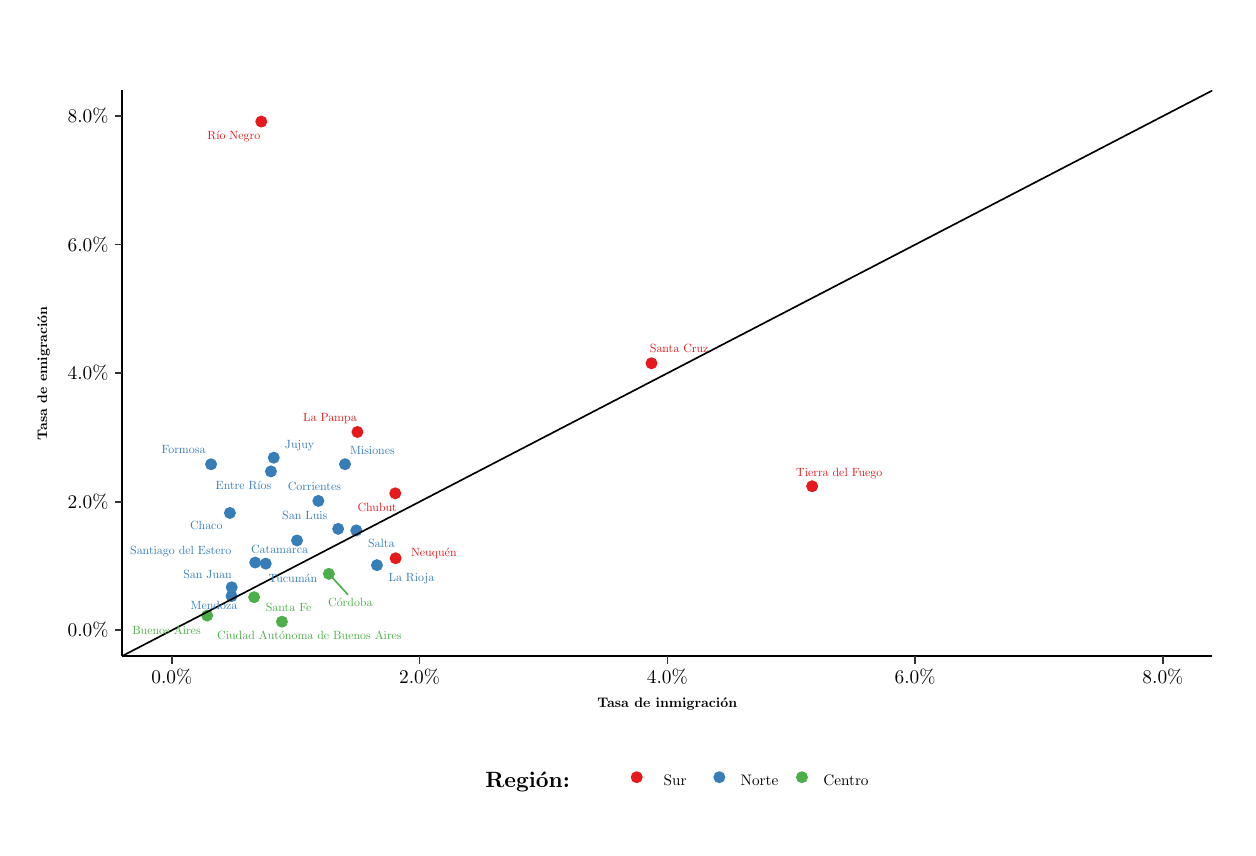
\begin{tikzpicture}[x=1pt,y=1pt]
\definecolor{fillColor}{RGB}{255,255,255}
\path[use as bounding box,fill=fillColor,fill opacity=0.00] (0,0) rectangle (433.62,289.08);
\begin{scope}
\path[clip] (  0.00,  0.00) rectangle (433.62,289.08);
\definecolor{drawColor}{RGB}{255,255,255}
\definecolor{fillColor}{RGB}{255,255,255}

\path[draw=drawColor,line width= 0.6pt,line join=round,line cap=round,fill=fillColor] (  0.00, -0.00) rectangle (433.62,289.08);
\end{scope}
\begin{scope}
\path[clip] ( 34.17, 62.03) rectangle (428.12,266.40);
\definecolor{drawColor}{RGB}{255,255,255}

\path[draw=drawColor,line width= 0.3pt,line join=round] ( 34.17, 94.54) --
	(428.12, 94.54);

\path[draw=drawColor,line width= 0.3pt,line join=round] ( 34.17,140.99) --
	(428.12,140.99);

\path[draw=drawColor,line width= 0.3pt,line join=round] ( 34.17,187.44) --
	(428.12,187.44);

\path[draw=drawColor,line width= 0.3pt,line join=round] ( 34.17,233.89) --
	(428.12,233.89);

\path[draw=drawColor,line width= 0.3pt,line join=round] ( 96.84, 62.03) --
	( 96.84,266.40);

\path[draw=drawColor,line width= 0.3pt,line join=round] (186.38, 62.03) --
	(186.38,266.40);

\path[draw=drawColor,line width= 0.3pt,line join=round] (275.91, 62.03) --
	(275.91,266.40);

\path[draw=drawColor,line width= 0.3pt,line join=round] (365.45, 62.03) --
	(365.45,266.40);

\path[draw=drawColor,line width= 0.6pt,line join=round] ( 34.17, 71.32) --
	(428.12, 71.32);

\path[draw=drawColor,line width= 0.6pt,line join=round] ( 34.17,117.77) --
	(428.12,117.77);

\path[draw=drawColor,line width= 0.6pt,line join=round] ( 34.17,164.22) --
	(428.12,164.22);

\path[draw=drawColor,line width= 0.6pt,line join=round] ( 34.17,210.67) --
	(428.12,210.67);

\path[draw=drawColor,line width= 0.6pt,line join=round] ( 34.17,257.11) --
	(428.12,257.11);

\path[draw=drawColor,line width= 0.6pt,line join=round] ( 52.07, 62.03) --
	( 52.07,266.40);

\path[draw=drawColor,line width= 0.6pt,line join=round] (141.61, 62.03) --
	(141.61,266.40);

\path[draw=drawColor,line width= 0.6pt,line join=round] (231.14, 62.03) --
	(231.14,266.40);

\path[draw=drawColor,line width= 0.6pt,line join=round] (320.68, 62.03) --
	(320.68,266.40);

\path[draw=drawColor,line width= 0.6pt,line join=round] (410.21, 62.03) --
	(410.21,266.40);
\definecolor{drawColor}{RGB}{77,175,74}
\definecolor{fillColor}{RGB}{77,175,74}

\path[draw=drawColor,line width= 0.4pt,line join=round,line cap=round,fill=fillColor] ( 64.86, 76.64) circle (  1.96);
\definecolor{drawColor}{RGB}{55,126,184}
\definecolor{fillColor}{RGB}{55,126,184}

\path[draw=drawColor,line width= 0.4pt,line join=round,line cap=round,fill=fillColor] ( 97.33,103.78) circle (  1.96);

\path[draw=drawColor,line width= 0.4pt,line join=round,line cap=round,fill=fillColor] ( 73.07,113.72) circle (  1.96);
\definecolor{drawColor}{RGB}{228,26,28}
\definecolor{fillColor}{RGB}{228,26,28}

\path[draw=drawColor,line width= 0.4pt,line join=round,line cap=round,fill=fillColor] (132.83,120.81) circle (  1.96);
\definecolor{drawColor}{RGB}{77,175,74}
\definecolor{fillColor}{RGB}{77,175,74}

\path[draw=drawColor,line width= 0.4pt,line join=round,line cap=round,fill=fillColor] ( 91.88, 74.43) circle (  1.96);

\path[draw=drawColor,line width= 0.4pt,line join=round,line cap=round,fill=fillColor] (108.83, 91.72) circle (  1.96);
\definecolor{drawColor}{RGB}{55,126,184}
\definecolor{fillColor}{RGB}{55,126,184}

\path[draw=drawColor,line width= 0.4pt,line join=round,line cap=round,fill=fillColor] (105.03,118.07) circle (  1.96);

\path[draw=drawColor,line width= 0.4pt,line join=round,line cap=round,fill=fillColor] ( 87.90,128.73) circle (  1.96);

\path[draw=drawColor,line width= 0.4pt,line join=round,line cap=round,fill=fillColor] ( 66.27,131.31) circle (  1.96);

\path[draw=drawColor,line width= 0.4pt,line join=round,line cap=round,fill=fillColor] ( 88.93,133.69) circle (  1.96);
\definecolor{drawColor}{RGB}{228,26,28}
\definecolor{fillColor}{RGB}{228,26,28}

\path[draw=drawColor,line width= 0.4pt,line join=round,line cap=round,fill=fillColor] (119.16,142.98) circle (  1.96);
\definecolor{drawColor}{RGB}{55,126,184}
\definecolor{fillColor}{RGB}{55,126,184}

\path[draw=drawColor,line width= 0.4pt,line join=round,line cap=round,fill=fillColor] (126.21, 94.86) circle (  1.96);

\path[draw=drawColor,line width= 0.4pt,line join=round,line cap=round,fill=fillColor] ( 73.68, 83.68) circle (  1.96);

\path[draw=drawColor,line width= 0.4pt,line join=round,line cap=round,fill=fillColor] (114.67,131.34) circle (  1.96);
\definecolor{drawColor}{RGB}{228,26,28}
\definecolor{fillColor}{RGB}{228,26,28}

\path[draw=drawColor,line width= 0.4pt,line join=round,line cap=round,fill=fillColor] (132.96, 97.34) circle (  1.96);

\path[draw=drawColor,line width= 0.4pt,line join=round,line cap=round,fill=fillColor] ( 84.42,255.15) circle (  1.96);
\definecolor{drawColor}{RGB}{55,126,184}
\definecolor{fillColor}{RGB}{55,126,184}

\path[draw=drawColor,line width= 0.4pt,line join=round,line cap=round,fill=fillColor] (118.74,107.41) circle (  1.96);

\path[draw=drawColor,line width= 0.4pt,line join=round,line cap=round,fill=fillColor] ( 73.73, 86.86) circle (  1.96);

\path[draw=drawColor,line width= 0.4pt,line join=round,line cap=round,fill=fillColor] (112.19,107.98) circle (  1.96);
\definecolor{drawColor}{RGB}{228,26,28}
\definecolor{fillColor}{RGB}{228,26,28}

\path[draw=drawColor,line width= 0.4pt,line join=round,line cap=round,fill=fillColor] (225.42,167.81) circle (  1.96);
\definecolor{drawColor}{RGB}{77,175,74}
\definecolor{fillColor}{RGB}{77,175,74}

\path[draw=drawColor,line width= 0.4pt,line join=round,line cap=round,fill=fillColor] ( 81.83, 83.28) circle (  1.96);
\definecolor{drawColor}{RGB}{55,126,184}
\definecolor{fillColor}{RGB}{55,126,184}

\path[draw=drawColor,line width= 0.4pt,line join=round,line cap=round,fill=fillColor] ( 82.22, 95.80) circle (  1.96);
\definecolor{drawColor}{RGB}{228,26,28}
\definecolor{fillColor}{RGB}{228,26,28}

\path[draw=drawColor,line width= 0.4pt,line join=round,line cap=round,fill=fillColor] (283.47,123.37) circle (  1.96);
\definecolor{drawColor}{RGB}{55,126,184}
\definecolor{fillColor}{RGB}{55,126,184}

\path[draw=drawColor,line width= 0.4pt,line join=round,line cap=round,fill=fillColor] ( 86.04, 95.41) circle (  1.96);
\definecolor{drawColor}{RGB}{0,0,0}

\path[draw=drawColor,line width= 0.6pt,line join=round] ( 34.17, 62.03) -- (428.12,266.40);
\definecolor{drawColor}{RGB}{77,175,74}

\path[draw=drawColor,line width= 0.6pt,line join=round,line cap=round] (115.67, 84.25) -- (109.36, 91.14);

\node[text=drawColor,anchor=base,inner sep=0pt, outer sep=0pt, scale=  0.43] at ( 50.17, 69.95) {Buenos Aires};
\definecolor{drawColor}{RGB}{55,126,184}

\node[text=drawColor,anchor=base,inner sep=0pt, outer sep=0pt, scale=  0.43] at ( 91.02, 98.95) {Catamarca};

\node[text=drawColor,anchor=base,inner sep=0pt, outer sep=0pt, scale=  0.43] at ( 64.53,107.78) {Chaco};
\definecolor{drawColor}{RGB}{228,26,28}

\node[text=drawColor,anchor=base,inner sep=0pt, outer sep=0pt, scale=  0.43] at (126.30,114.20) {Chubut};
\definecolor{drawColor}{RGB}{77,175,74}

\node[text=drawColor,anchor=base,inner sep=0pt, outer sep=0pt, scale=  0.43] at (101.81, 67.84) {Ciudad Autónoma de Buenos Aires};

\node[text=drawColor,anchor=base,inner sep=0pt, outer sep=0pt, scale=  0.43] at (116.60, 79.81) {Córdoba};
\definecolor{drawColor}{RGB}{55,126,184}

\node[text=drawColor,anchor=base,inner sep=0pt, outer sep=0pt, scale=  0.43] at (103.62,121.74) {Corrientes};

\node[text=drawColor,anchor=base,inner sep=0pt, outer sep=0pt, scale=  0.43] at ( 77.98,122.10) {Entre Ríos};

\node[text=drawColor,anchor=base,inner sep=0pt, outer sep=0pt, scale=  0.43] at ( 56.31,135.03) {Formosa};

\node[text=drawColor,anchor=base,inner sep=0pt, outer sep=0pt, scale=  0.43] at ( 98.25,137.03) {Jujuy};
\definecolor{drawColor}{RGB}{228,26,28}

\node[text=drawColor,anchor=base,inner sep=0pt, outer sep=0pt, scale=  0.43] at (109.22,146.69) {La Pampa};
\definecolor{drawColor}{RGB}{55,126,184}

\node[text=drawColor,anchor=base,inner sep=0pt, outer sep=0pt, scale=  0.43] at (138.68, 88.82) {La Rioja};

\node[text=drawColor,anchor=base,inner sep=0pt, outer sep=0pt, scale=  0.43] at ( 67.31, 78.90) {Mendoza};

\node[text=drawColor,anchor=base,inner sep=0pt, outer sep=0pt, scale=  0.43] at (124.59,135.02) {Misiones};
\definecolor{drawColor}{RGB}{228,26,28}

\node[text=drawColor,anchor=base,inner sep=0pt, outer sep=0pt, scale=  0.43] at (146.76, 97.81) {Neuquén};

\node[text=drawColor,anchor=base,inner sep=0pt, outer sep=0pt, scale=  0.43] at ( 74.51,248.52) {Río Negro};
\definecolor{drawColor}{RGB}{55,126,184}

\node[text=drawColor,anchor=base,inner sep=0pt, outer sep=0pt, scale=  0.43] at (127.77,101.23) {Salta};

\node[text=drawColor,anchor=base,inner sep=0pt, outer sep=0pt, scale=  0.43] at ( 65.00, 89.96) {San Juan};

\node[text=drawColor,anchor=base,inner sep=0pt, outer sep=0pt, scale=  0.43] at (100.14,111.41) {San Luis};
\definecolor{drawColor}{RGB}{228,26,28}

\node[text=drawColor,anchor=base,inner sep=0pt, outer sep=0pt, scale=  0.43] at (235.42,171.53) {Santa Cruz};
\definecolor{drawColor}{RGB}{77,175,74}

\node[text=drawColor,anchor=base,inner sep=0pt, outer sep=0pt, scale=  0.43] at ( 94.29, 78.20) {Santa Fe};
\definecolor{drawColor}{RGB}{55,126,184}

\node[text=drawColor,anchor=base,inner sep=0pt, outer sep=0pt, scale=  0.43] at ( 55.30, 98.88) {Santiago del Estero};
\definecolor{drawColor}{RGB}{228,26,28}

\node[text=drawColor,anchor=base,inner sep=0pt, outer sep=0pt, scale=  0.43] at (293.27,127.02) {Tierra del Fuego};
\definecolor{drawColor}{RGB}{55,126,184}

\node[text=drawColor,anchor=base,inner sep=0pt, outer sep=0pt, scale=  0.43] at ( 95.86, 88.77) {Tucumán};
\end{scope}
\begin{scope}
\path[clip] (  0.00,  0.00) rectangle (433.62,289.08);
\definecolor{drawColor}{RGB}{0,0,0}

\path[draw=drawColor,line width= 0.6pt,line join=round] ( 34.17, 62.03) --
	( 34.17,266.40);
\end{scope}
\begin{scope}
\path[clip] (  0.00,  0.00) rectangle (433.62,289.08);
\definecolor{drawColor}{RGB}{0,0,0}

\node[text=drawColor,anchor=base east,inner sep=0pt, outer sep=0pt, scale=  0.70] at ( 29.22, 68.91) {0.0{\%}};

\node[text=drawColor,anchor=base east,inner sep=0pt, outer sep=0pt, scale=  0.70] at ( 29.22,115.36) {2.0{\%}};

\node[text=drawColor,anchor=base east,inner sep=0pt, outer sep=0pt, scale=  0.70] at ( 29.22,161.81) {4.0{\%}};

\node[text=drawColor,anchor=base east,inner sep=0pt, outer sep=0pt, scale=  0.70] at ( 29.22,208.25) {6.0{\%}};

\node[text=drawColor,anchor=base east,inner sep=0pt, outer sep=0pt, scale=  0.70] at ( 29.22,254.70) {8.0{\%}};
\end{scope}
\begin{scope}
\path[clip] (  0.00,  0.00) rectangle (433.62,289.08);
\definecolor{drawColor}{gray}{0.20}

\path[draw=drawColor,line width= 0.6pt,line join=round] ( 31.42, 71.32) --
	( 34.17, 71.32);

\path[draw=drawColor,line width= 0.6pt,line join=round] ( 31.42,117.77) --
	( 34.17,117.77);

\path[draw=drawColor,line width= 0.6pt,line join=round] ( 31.42,164.22) --
	( 34.17,164.22);

\path[draw=drawColor,line width= 0.6pt,line join=round] ( 31.42,210.67) --
	( 34.17,210.67);

\path[draw=drawColor,line width= 0.6pt,line join=round] ( 31.42,257.11) --
	( 34.17,257.11);
\end{scope}
\begin{scope}
\path[clip] (  0.00,  0.00) rectangle (433.62,289.08);
\definecolor{drawColor}{RGB}{0,0,0}

\path[draw=drawColor,line width= 0.6pt,line join=round] ( 34.17, 62.03) --
	(428.12, 62.03);
\end{scope}
\begin{scope}
\path[clip] (  0.00,  0.00) rectangle (433.62,289.08);
\definecolor{drawColor}{gray}{0.20}

\path[draw=drawColor,line width= 0.6pt,line join=round] ( 52.07, 59.28) --
	( 52.07, 62.03);

\path[draw=drawColor,line width= 0.6pt,line join=round] (141.61, 59.28) --
	(141.61, 62.03);

\path[draw=drawColor,line width= 0.6pt,line join=round] (231.14, 59.28) --
	(231.14, 62.03);

\path[draw=drawColor,line width= 0.6pt,line join=round] (320.68, 59.28) --
	(320.68, 62.03);

\path[draw=drawColor,line width= 0.6pt,line join=round] (410.21, 59.28) --
	(410.21, 62.03);
\end{scope}
\begin{scope}
\path[clip] (  0.00,  0.00) rectangle (433.62,289.08);
\definecolor{drawColor}{RGB}{0,0,0}

\node[text=drawColor,anchor=base,inner sep=0pt, outer sep=0pt, scale=  0.70] at ( 52.07, 52.26) {0.0{\%}};

\node[text=drawColor,anchor=base,inner sep=0pt, outer sep=0pt, scale=  0.70] at (141.61, 52.26) {2.0{\%}};

\node[text=drawColor,anchor=base,inner sep=0pt, outer sep=0pt, scale=  0.70] at (231.14, 52.26) {4.0{\%}};

\node[text=drawColor,anchor=base,inner sep=0pt, outer sep=0pt, scale=  0.70] at (320.68, 52.26) {6.0{\%}};

\node[text=drawColor,anchor=base,inner sep=0pt, outer sep=0pt, scale=  0.70] at (410.21, 52.26) {8.0{\%}};
\end{scope}
\begin{scope}
\path[clip] (  0.00,  0.00) rectangle (433.62,289.08);
\definecolor{drawColor}{RGB}{0,0,0}

\node[text=drawColor,anchor=base,inner sep=0pt, outer sep=0pt, scale=  0.50] at (231.14, 43.31) {\bfseries Tasa de inmigración};
\end{scope}
\begin{scope}
\path[clip] (  0.00,  0.00) rectangle (433.62,289.08);
\definecolor{drawColor}{RGB}{0,0,0}

\node[text=drawColor,rotate= 90.00,anchor=base,inner sep=0pt, outer sep=0pt, scale=  0.50] at ( 7,164.22) {\bfseries Tasa de emigración};
\end{scope}
\begin{scope}
\path[clip] (  0.00,  0.00) rectangle (433.62,289.08);
\definecolor{fillColor}{RGB}{255,255,255}

\path[fill=fillColor] (159.87,  5.50) rectangle (302.41, 30.95);
\end{scope}
\begin{scope}
\path[clip] (  0.00,  0.00) rectangle (433.62,289.08);
\definecolor{drawColor}{RGB}{0,0,0}

\node[text=drawColor,anchor=base west,inner sep=0pt, outer sep=0pt, scale=  0.80] at (165.37, 14.43) {\bfseries Región:};
\end{scope}
\begin{scope}
\path[clip] (  0.00,  0.00) rectangle (433.62,289.08);
\definecolor{drawColor}{RGB}{228,26,28}
\definecolor{fillColor}{RGB}{228,26,28}

\path[draw=drawColor,line width= 0.4pt,line join=round,line cap=round,fill=fillColor] (220.08, 18.23) circle (  1.96);
\end{scope}
\begin{scope}
\path[clip] (  0.00,  0.00) rectangle (433.62,289.08);
\definecolor{drawColor}{RGB}{55,126,184}
\definecolor{fillColor}{RGB}{55,126,184}

\path[draw=drawColor,line width= 0.4pt,line join=round,line cap=round,fill=fillColor] (249.93, 18.23) circle (  1.96);
\end{scope}
\begin{scope}
\path[clip] (  0.00,  0.00) rectangle (433.62,289.08);
\definecolor{drawColor}{RGB}{77,175,74}
\definecolor{fillColor}{RGB}{77,175,74}

\path[draw=drawColor,line width= 0.4pt,line join=round,line cap=round,fill=fillColor] (279.79, 18.23) circle (  1.96);
\end{scope}
\begin{scope}
\path[clip] (  0.00,  0.00) rectangle (433.62,289.08);
\definecolor{drawColor}{RGB}{0,0,0}

\node[text=drawColor,anchor=base west,inner sep=0pt, outer sep=0pt, scale=  0.55] at (229.81, 15.20) {Sur};
\end{scope}
\begin{scope}
\path[clip] (  0.00,  0.00) rectangle (433.62,289.08);
\definecolor{drawColor}{RGB}{0,0,0}

\node[text=drawColor,anchor=base west,inner sep=0pt, outer sep=0pt, scale=  0.55] at (257.66, 15.20) {Norte};
\end{scope}
\begin{scope}
\path[clip] (  0.00,  0.00) rectangle (433.62,289.08);
\definecolor{drawColor}{RGB}{0,0,0}

\node[text=drawColor,anchor=base west,inner sep=0pt, outer sep=0pt, scale=  0.55] at (287.51, 15.20) {Centro};
\end{scope}
\end{tikzpicture}
